\documentclass[]{standalone}

\begin{document}
	\begin{frame}{Tissue Segmentation}{A Gaussian Mixture model approach.}
	
	\vspace{-25pt}
		\begin{columns}
			\begin{column}{0.4\textwidth}
				\begin{itemize}
				\item Find Tissues Mean Values and Weights;
				\item Define a Gaussian Mixture Model;
				\item Expectation Maximization;
				\item Classification.
				\end{itemize}
			\end{column}
			\begin{column}{0.7\textwidth}
			\begin{figure}[h!]
			\centering
			%\vspace{-6pt}

				\begin{subfigure}{0.45\textwidth}
					
					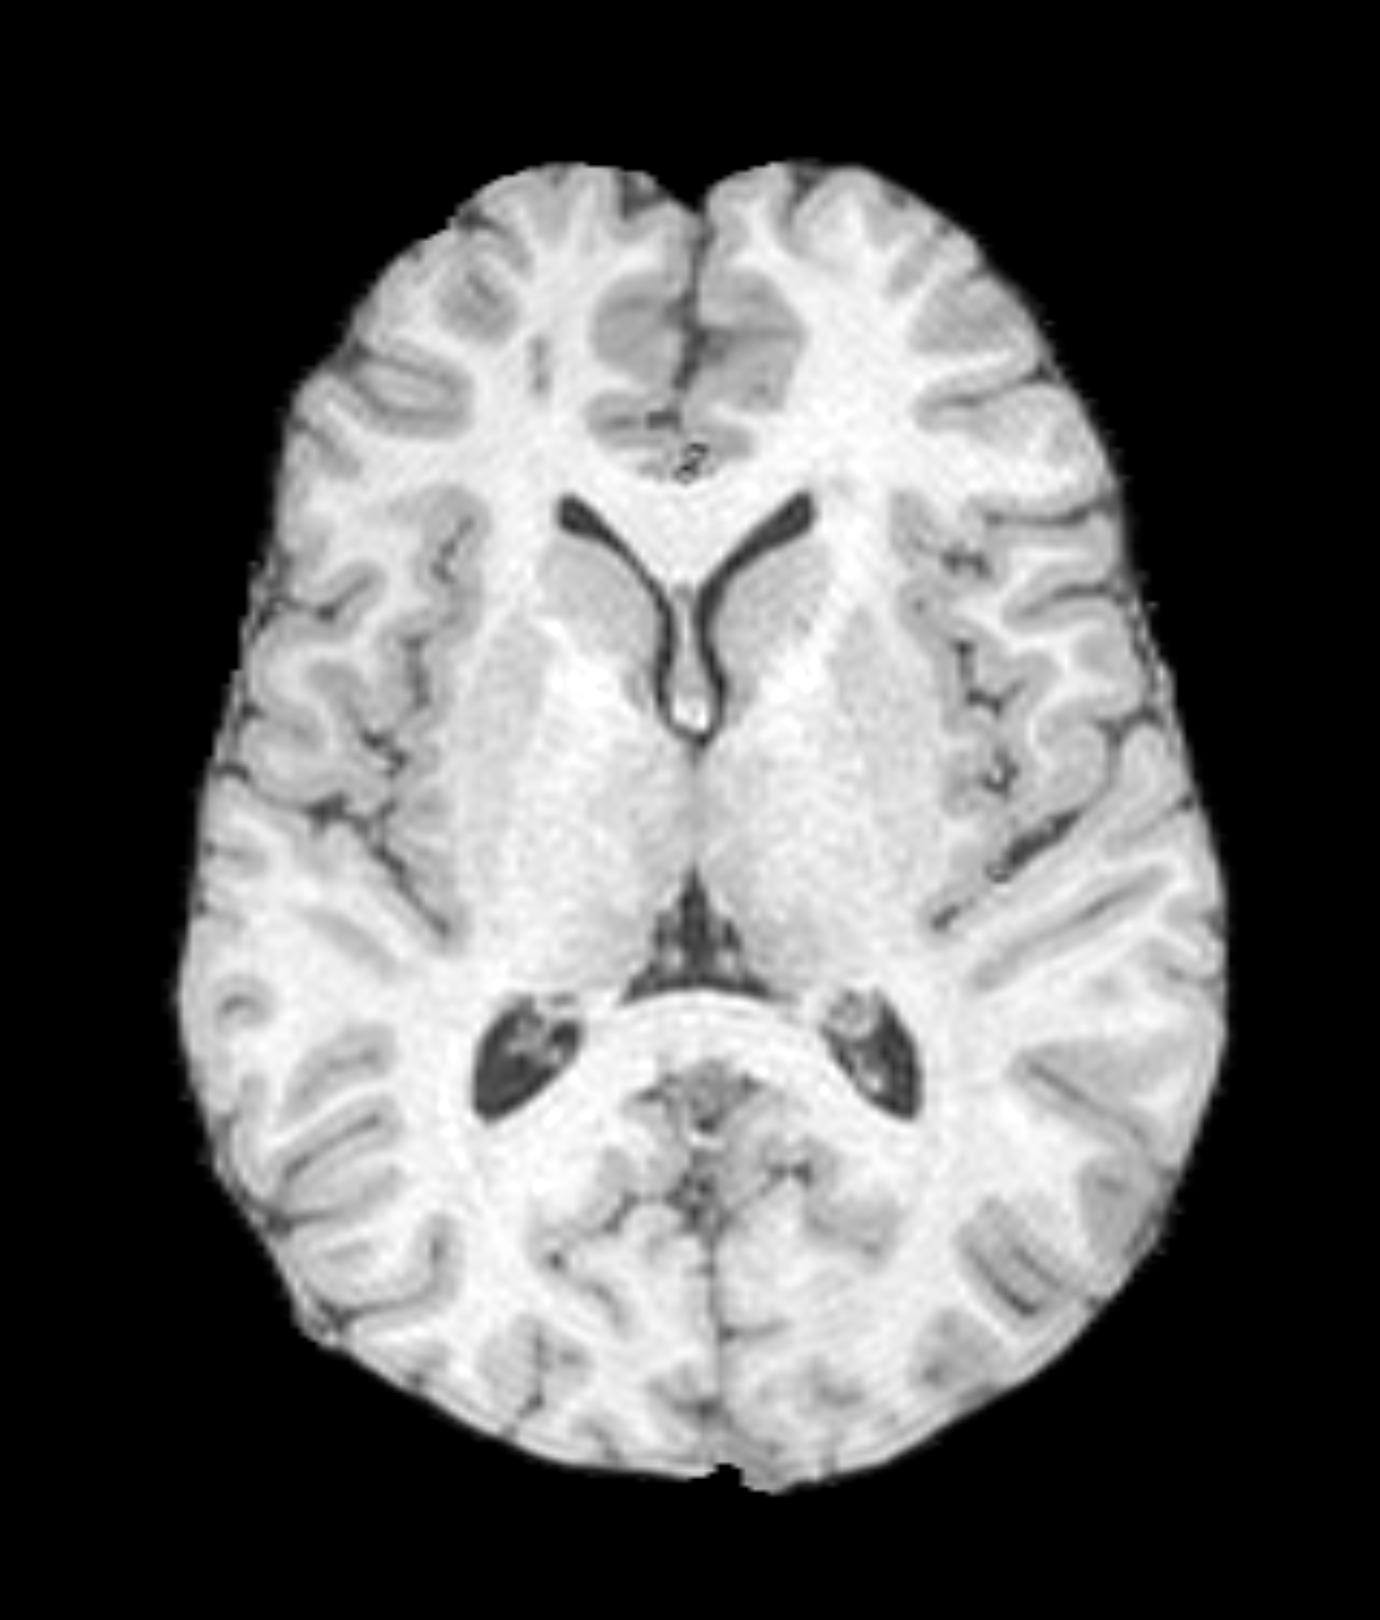
\includegraphics[scale=0.0551]{./IMG/brain.jpg}
				\end{subfigure}
				\hspace{15pt} %so che è strano ma è l'unico modo di farlo venire benino...
				\hspace{-48pt}
				\begin{subfigure}{0.45\textwidth}
					
					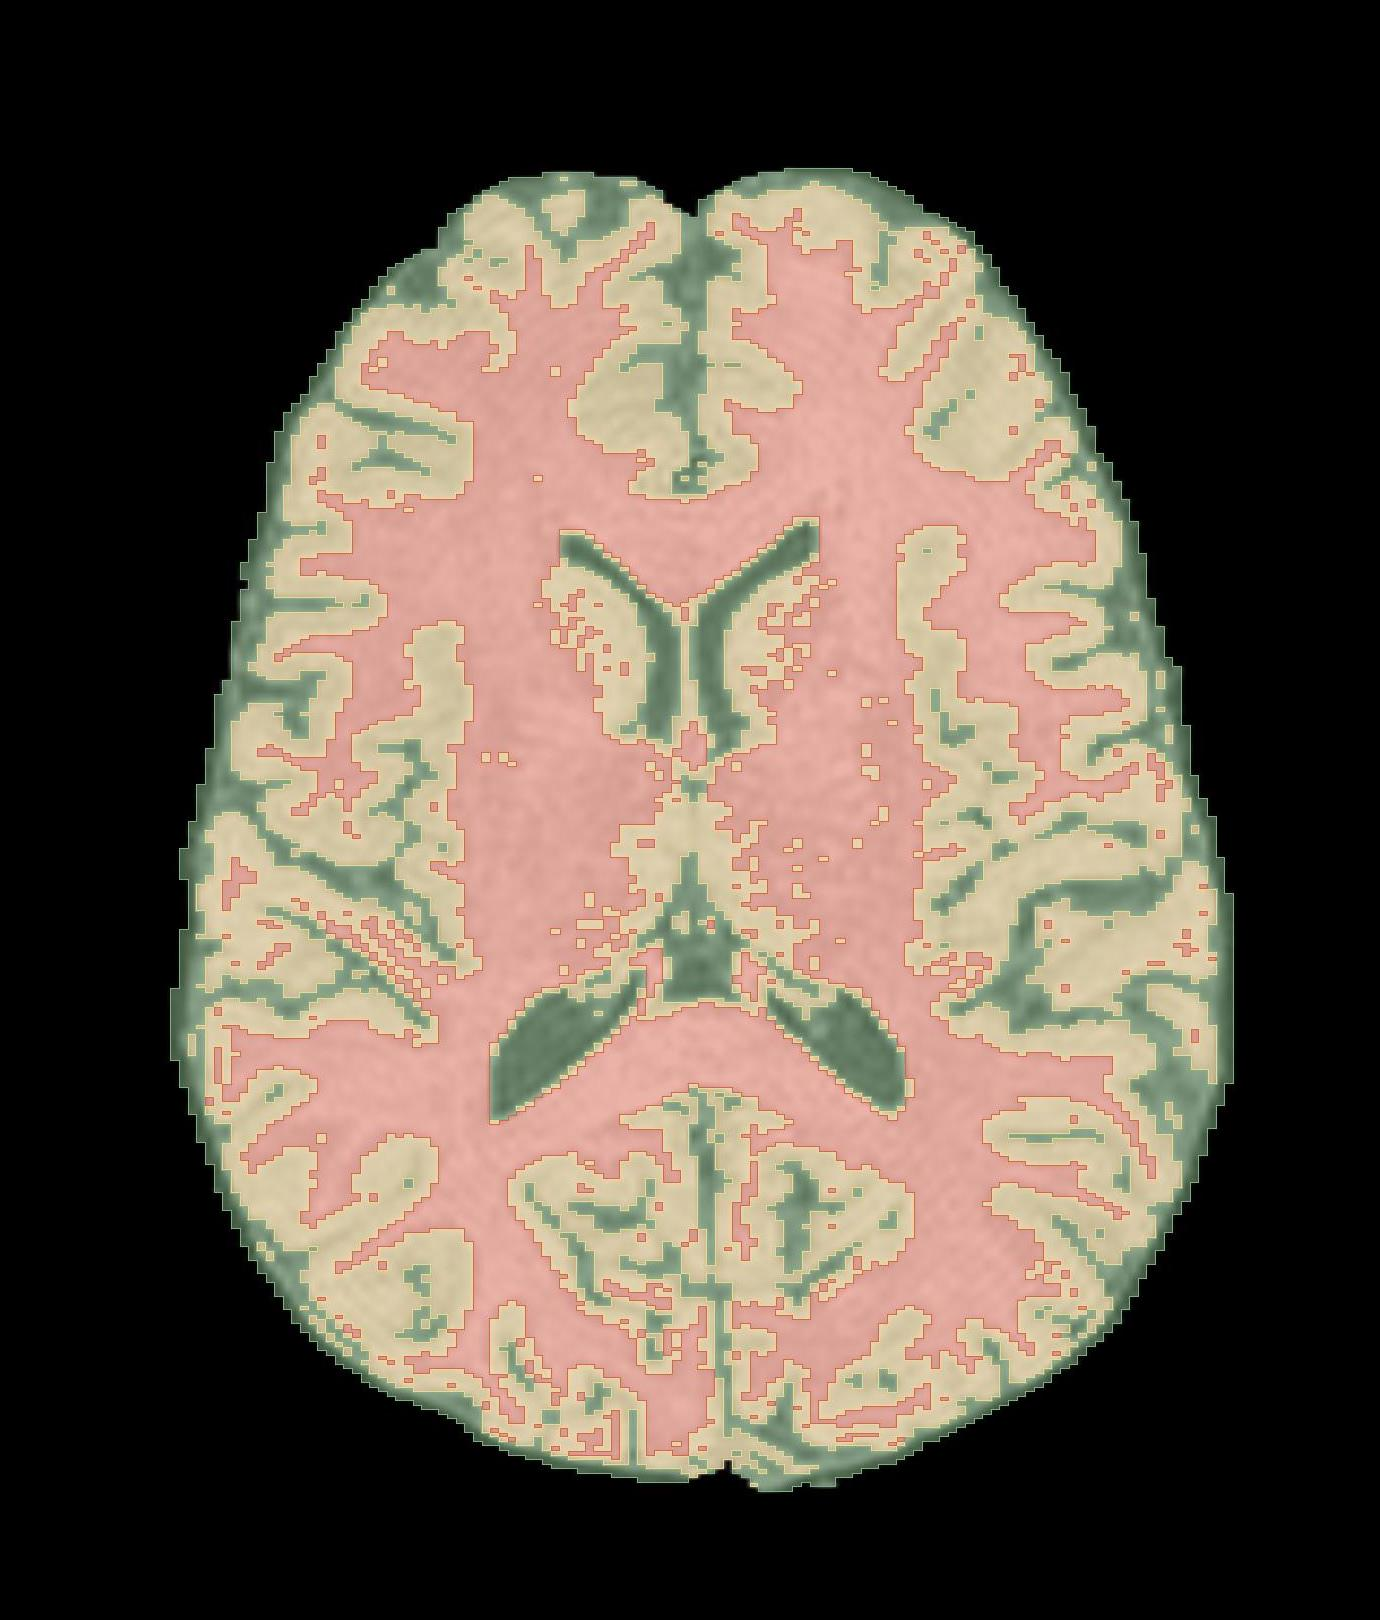
\includegraphics[scale=0.055]{./IMG/segmented_axial.jpg}
				\end{subfigure}
				\hfill
				\begin{subfigure}{0.45\textwidth}
					
					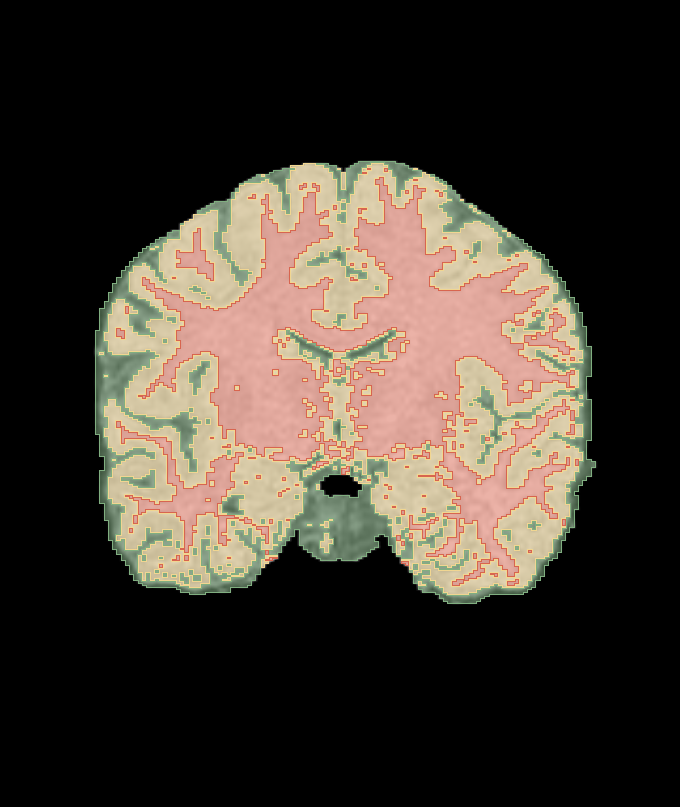
\includegraphics[scale=0.112]{./IMG/segmented_frontal.png}
				\end{subfigure}
				\hspace{15pt}
				\hspace{-48pt}
				\begin{subfigure}{0.45\textwidth}
					
					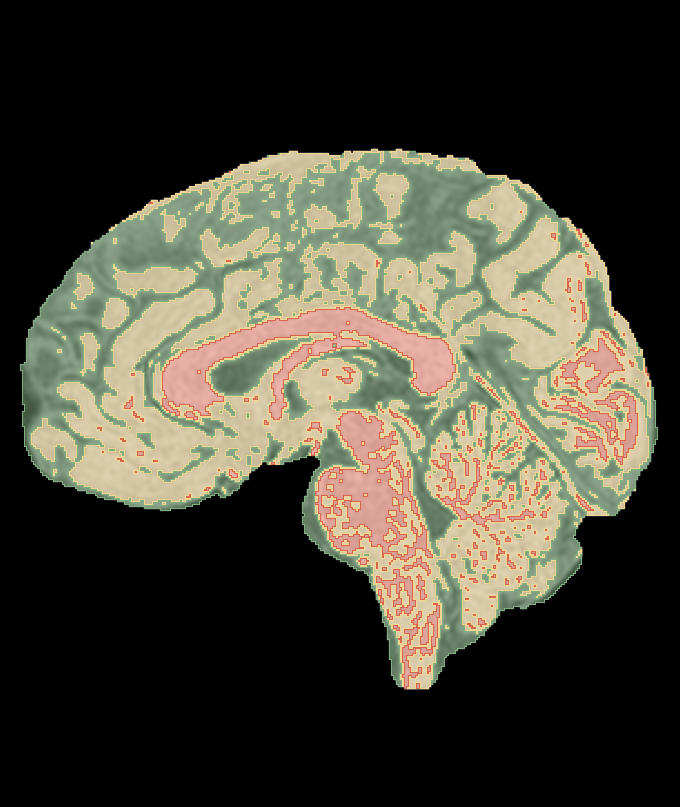
\includegraphics[scale=0.112]{./IMG/segmented_lateral.png}
				\end{subfigure}

			\end{figure}
			\end{column}
		\end{columns}
	\end{frame}
\end{document}
